%%%%%%%%%%%%%%%%%%%%%%%%%%%%%%%%%%%%%%%%%%%%%%%%%%%%%
% 緒言
%%%%%%%%%%%%%%%%%%%%%%%%%%%%%%%%%%%%%%%%%%%%%%%%%%%%%

\chapter{緒言}
\label{Chapter1}

\section{本論文の構成}\label{Sec:sub_introduction}

緒言を書こう~\cite{bibtest}.

図の参照テスト Fig.~\ref{fig:test}.%reffig使うと太字になります


\begin{figure}[tb]
    \centering 
     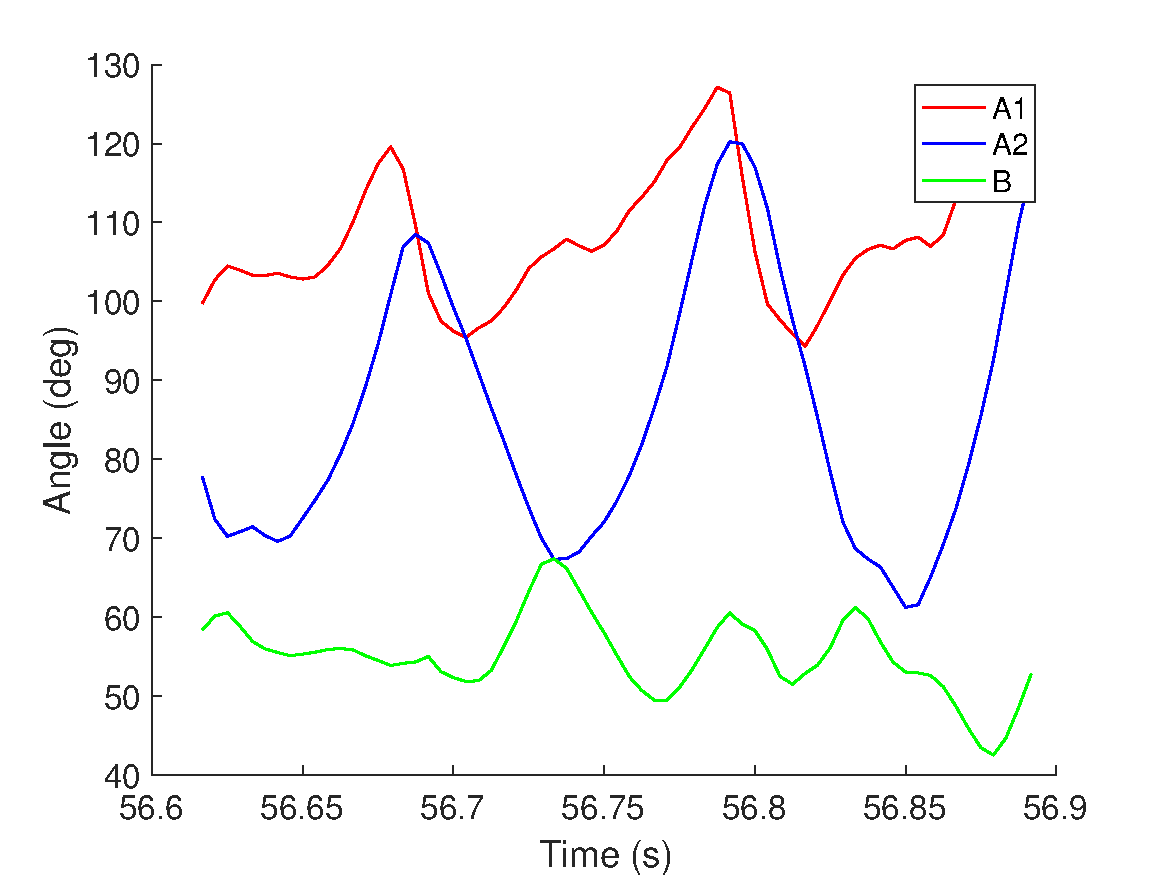
\includegraphics[width=\columnwidth]{./figure/testfig.pdf}
     \caption{キャプションを書こう}
     \label{fig:test}
\end{figure}

\begin{align}
    y=\sin{A}
    \label{eq:test}
\end{align}


現代社会において,屋内で移動や作業をするロボットが様々な場面で必要とされているのは言うまでも無い.
その際の移動方法としては移動用クローラ~\cite{小柳栄次2010サブクローラを持つレスキューロボット}や車輪~\cite{尾崎功一20082p2}を利用したものなどがある.
これらの移動ロボットは地面の凹凸などに柔軟に対応し,高い踏破性を持つが,人間が生活するような屋内を移動する上では,階段などの段差が大きな障害となる.
クローラ型のロボットの中にはそういった段差の問題を,2つのクローラ機構を有することによって解決している物もあるが~\cite{小柳栄次2010サブクローラを持つレスキューロボット},越えることのできる段差の大きさがクローラの大きさに依存してしまうという課題を抱えている.
移動機構が大きくなるということは,結果的にそのロボットの活動範囲を縮めてしまうことになる.そこで,移動機構の大きさに依存せず,段差を踏破できるロボットを開発することで,活動範囲を縮めずに屋内の移動をするロボットの開発を目指す.
本研究では,そのような移動機構を持つロボットの1つとして壁面歩行ロボットの開発を行う.

階段のような段差も広く捉えれば壁であり,その壁面に吸着し移動することで,段差などの踏破を実現できる.
また,凹凸や亀裂など壁面の状況によっては吸着による移動が難しい場合もある.
そこで,凹凸などへも対応できる吸着機構の開発を目指しつつ,吸着がどうしても不可能な段差に対しては,屋内の別の壁面を利用することで,段差を利用せずに目的地にたどり着くなど,様々なルートの選択が可能になるロボットの開発ができればより有用である.

今日に至るまで壁面歩行ロボットというのは様々な形で実現されてきた.
その吸着機構としては,吸盤などの負圧を利用するもの~\cite{広瀬茂男1991四足壁面移動ロボット},磁力を利用するもの~\cite{高田洋吾2013立体的な環境で活動できる橋梁検査ロボットの開発},プロペラなどによる推進力を利用するもの~\cite{weko_4205_1}などがある.
磁力式は強力な吸着力によって磁性を持つ平面上での作業ロボットとして有用である~\cite{高田洋吾2013立体的な環境で活動できる橋梁検査ロボットの開発}.しかし,吸着できる面が磁性を持つものに限られるという課題がある.
また,推進力式は移動の速さに利点があるが~\cite{weko_4205_1},吸着の安定のための制御器への負担と,風などの外部環境の影響を受けることに課題がある~\cite{西亮1991推進力による壁面移動ロボットの研究,鈴木隆宏2009g1501}.
よって本研究においては,吸着面の材質を選ばず,吸着面との気密性を保つことができれば,安定的な吸着力を発揮することのできる負圧式を吸着機構として選択した.

現存する負圧式の壁面歩行ロボットは,その移動方法を大きく吸着式クローラ型~\cite{福田敏男1994壁面走行ロボットの研究}と脚型~\cite{広瀬茂男1991四足壁面移動ロボット}に分けることができる.
一般に,吸着式クローラ型は移動速度において脚型よりも優れているが\cite{福田敏男1992壁面走行ロボッ},脚型は脚の接地面を選択できるので,吸着のしにくい凹凸や亀裂を避けて移動することができる.
以上のことから本研究では負圧による吸着機構を有する脚型の壁面歩行ロボットの製作を目指す.
その壁面歩行ロボット製作に向けてまずは,壁面のみを移動することのできる脚型壁面歩行ロボットの開発と性能実験に取り組んだ.




